\documentclass[preprint,12pt,aps,pra,showkeys,amsmath,amssymb,superscriptaddress,floatfix]{revtex4-2}
\usepackage[T1]{fontenc}
\usepackage[utf8]{inputenc}
\usepackage{amsmath,amssymb,amsthm,mathtools,mathrsfs}
\usepackage{microtype,booktabs,enumitem}
\usepackage{xcolor,tikz,etoolbox}
\usepackage[skins,breakable]{tcolorbox}
\usepackage{needspace}
% Keep diagram geometry independent of REVTeX preprint body spacing.
\AtBeginEnvironment{tikzpicture}{\linespread{1}\selectfont}
\usetikzlibrary{arrows.meta,positioning,calc,fit,decorations.pathreplacing}
\usepackage{graphicx}
\usepackage{hyperref}

\definecolor{MMBlue}{RGB}{0,82,155}
\definecolor{MMOrange}{RGB}{200,80,0}
\tikzset{
 mmnode/.style={draw=MMBlue,rounded corners=2pt,fill=MMBlue!4,align=left,execute at begin node={\raggedright},text width=5cm,font=\fontsize{10}{12}\selectfont,inner sep=6pt},
 mmimport/.style={mmnode,draw=black!65,fill=black!4},
 mmcandidate/.style={mmnode,draw=MMOrange,dashed,fill=MMOrange!5},
 mmrejected/.style={mmnode,draw=black,densely dotted,fill=black!8},
 mmproof/.style={->,thick,MMBlue},
 mmflow/.style={->,semithick,black!70},
 mmrepair/.style={->,dashed,thick,MMOrange},
 mmcandidatearrow/.style={->,dashed,semithick,MMOrange},
 mmnote/.style={font=\scriptsize,fill=white,inner sep=2pt,align=center}}

\usepackage[section]{placeins}
\setlength{\emergencystretch}{3em}
\setlist{itemsep=3pt,topsep=4pt}
\newtheorem{theorem}{Theorem}[section]
\newtheorem{proposition}[theorem]{Proposition}
\newtheorem{lemma}[theorem]{Lemma}
\newtheorem{corollary}[theorem]{Corollary}
\theoremstyle{definition}
\newtheorem{definition}[theorem]{Definition}
\newtheorem{example}[theorem]{Example}
\theoremstyle{remark}
\newtheorem{remark}[theorem]{Remark}
% Avoid isolated statement headings and single-line paragraph fragments.
\BeforeBeginEnvironment{theorem}{\Needspace{6\baselineskip}}
\BeforeBeginEnvironment{definition}{\Needspace{5\baselineskip}}
\BeforeBeginEnvironment{proposition}{\Needspace{5\baselineskip}}
\BeforeBeginEnvironment{lemma}{\Needspace{5\baselineskip}}
\BeforeBeginEnvironment{corollary}{\Needspace{5\baselineskip}}
\clubpenalty=5000
\widowpenalty=5000
\newcommand{\R}{\mathbb R}\newcommand{\Z}{\mathbb Z}\newcommand{\N}{\mathbb N}
\newcommand{\Pa}{\operatorname{Pa}}\newcommand{\Desc}{\operatorname{Desc}}
\newcommand{\cl}{\operatorname{cl}}\newcommand{\cost}{\operatorname{cost}}
\newcommand{\status}{\operatorname{status}}
% Faculty cards: a visual rail groups the five faculties within one agent.
% The rail has no arrowhead and does not represent a proof dependency.
\newcommand{\mmfacultybadge}[1]{%
 \node[circle,draw=MMBlue,line width=1pt,fill=white,
 minimum size=7mm,inner sep=0pt,font=\sffamily\small\bfseries,text=MMBlue]
 at ([xshift=15pt,yshift=-15pt]frame.north west) {#1};}
\newcommand{\mmfacultyrail}{%
 \draw[MMBlue!80,line width=1pt]
 ([xshift=15pt,yshift=2pt]frame.north west)--
 ([xshift=15pt,yshift=-2pt]frame.south west);}
\newtcolorbox{mmfacultybox}[2]{enhanced,breakable,
 colback=MMBlue!4,colframe=MMBlue!4,boxrule=0pt,arc=3pt,
 left=39pt,right=9pt,top=4pt,bottom=4pt,
 before skip=2pt,after skip=2pt,
 fontupper=\small\linespread{1.1}\selectfont,
 overlay unbroken={\mmfacultyrail\mmfacultybadge{#1}},
 overlay first={\mmfacultyrail\mmfacultybadge{#1}},
 overlay middle={\mmfacultyrail},overlay last={\mmfacultyrail}}
\newcommand{\mmfaculty}[3]{%
 \begin{mmfacultybox}{#1}{#2}
 {\sffamily\bfseries\color{MMBlue}#2}\par\smallskip #3
 \end{mmfacultybox}}
\newcommand{\agent}[9]{%
 \Needspace{8\baselineskip}
 \subsubsection{#1}
 \noindent\textbf{Object.} #2\par
 \noindent\textbf{Role.} #3\par\smallskip
 \mmfaculty{E}{Ego}{#4}
 \mmfaculty{M}{Memory}{#5}
 \mmfaculty{I}{Intellect}{#6}
 \mmfaculty{S}{Sense}{#7}
 \mmfaculty{A}{Action}{#8}
 \smallskip\noindent #9\par}

\usepackage{longtable,array,calc}
\providecommand{\tightlist}{\setlength{\itemsep}{2pt}\setlength{\parskip}{0pt}}
\makeatletter
\def\frontmatter@abstract@produce{\par\addvspace{\frontmatter@preabstractspace}%
\begingroup\prep@absbox\unvbox\absbox\post@absbox\endgroup
\addvspace{\frontmatter@postabstractspace}}
\makeatother
\newcommand{\field}[2]{\par\smallskip\noindent\textbf{#1.} #2\par}
\setlength{\emergencystretch}{5em}
\AtBeginEnvironment{verbatim}{\small\linespread{1.0}\selectfont}


\hypersetup{colorlinks=true,linkcolor=MMBlue,urlcolor=MMBlue,pdfauthor={Dibakar Sigdel}}

\begin{document}

\title{Fundamental Theorem of Calculus\\[4pt]\large An End-to-End Meta-Math Walkthrough}

\author{Dibakar Sigdel}

\affiliation{Mindverse Computing LLC, Lynnwood, WA 98087, USA}

\date{October 2026}

\begin{abstract}

A complete authored walkthrough of fundamental theorem of calculus, with
explicit mathematical contracts, local verification gates, and reusable
exports. The report presents the target theorem, declared imports, a
dependency graph, five-faculty node contracts, a continuous proof, a
worked example, and a hypothesis-repair audit. It is an authored
mathematical exposition, not a deployed-agent transcript or a formal
proof-assistant certificate.

\end{abstract}\maketitle\linespread{1.12}\selectfont

\noindent\textbf{AC-02 / Advanced Calculus / Report v1}

\section{Target and import contract}

\begin{theorem}

For continuous \(f:[a,b]\to\mathbb R\), prove \(F(x)=\int_a^x f(t)\,dt\)
is differentiable on \((a,b)\) with \(F'=f\). If \(G'=f\) there and
\(G\) is continuous on \([a,b]\), prove \(\int_a^b f=G(b)-G(a)\).

\end{theorem}

\subsection{Foundations and permitted imports}

Use Riemann integrability of continuous functions on{[}a,b{]},
additivity and integral bounds, and AC-01. An integral with reversed
endpoints changes sign. Derivatives of accumulated integrals are taken
on (a,b), with one-sided endpoint continuity.

\clearpage\section{Node interaction workflow}

\begin{center}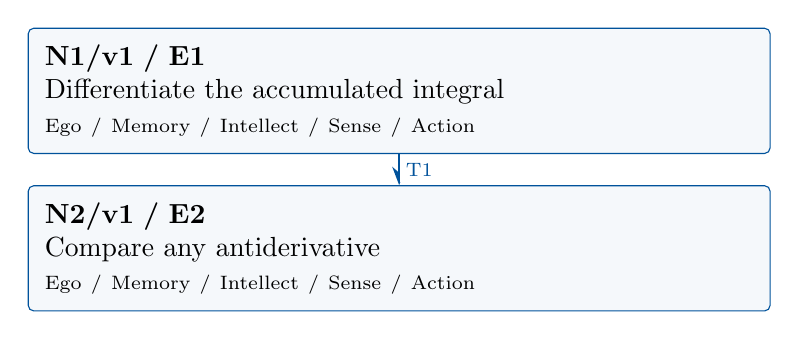
\begin{tikzpicture}[>=Stealth,x=1cm,y=1cm]

\node[mmnode,text width=9cm,minimum height=1.25cm] (N1) at (0,0.0) {\textbf{N1/v1 / E1}\\Differentiate the accumulated integral\\{\scriptsize Ego / Memory / Intellect / Sense / Action}};

\node[mmnode,text width=9cm,minimum height=1.25cm] (N2) at (0,-2.0) {\textbf{N2/v1 / E2}\\Compare any antiderivative\\{\scriptsize Ego / Memory / Intellect / Sense / Action}};

\draw[mmproof] (N1.south) -- node[mmnote,right] {T1} (N2.north);

\end{tikzpicture}\end{center}

Each box is one mathematical agent containing all five faculties. Blue
arrows carry the versioned exports listed below. The layout gives a
reading order; only drawn arrows assert dependencies. Diagnostic repair
is separate from the proof DAG.

\subsection{Versioned evidence-transfer ledger}

\begingroup\small\linespread{1.05}\selectfont

\Needspace{5\baselineskip}\field{T1: N1/E1/v1 to N2}{F is continuous on{[}a,b{]} and differentiable inside with \(F'=f\).}

\field{Receiving activity}{N2: Compare any antiderivative}

\field{Compatibility}{Use the same mathematical objects and hypotheses as the source export.
Receiving contract: \(G'=f\) inside and G continuous on{[}a,b{]}; prior
exports E1/v1}

\endgroup

\clearpage\section{Agent roles and five-faculty activities}\begingroup\small\linespread{1.05}\selectfont\setlist{itemsep=1pt,topsep=2pt}

\subsection{N1/v1: Differentiate the accumulated integral}

\field{Object and role}{Estimate the difference between a local average and \(f(x)\).}

\field{Inputs}{Continuous f; \(F(x)=\int _a^x\) f; foundational imports stated in §1}

\mmfaculty{E}{Ego}{Own E1/v1: F is continuous on{[}a,b{]} and differentiable inside with
\(F'=f\).}

\mmfaculty{M}{Memory}{Retain Continuous f; \(F(x)=\int _a^x\) f; foundational imports stated
in §1; keep their assumptions and versions attached.}

\mmfaculty{I}{Intellect}{Estimate the difference between a local average and \(f(x)\).}

\mmfaculty{S}{Sense}{For negative h, the reversed interval must be treated consistently.}

\mmfaculty{A}{Action}{Carry out the numbered deductions and publish E1/v1 together with its
hypotheses and proof location.}

\smallskip\noindent\textbf{Numbered mathematical activities}

\begin{enumerate}[label=N1.\arabic*,leftmargin=3.4em]

\item For x interior and sufficiently small nonzero h, additivity gives
\((F(x+h)-F(x))/h=(1/h)\int _x^{x+h}f(t)dt\).

\item Subtract \(f(x)\); the absolute difference is bounded by sup between x
andx+h \(of|f(t)-f(x)|\), including \(h<0\) using reversed integration.

\item Continuity makes this bound tend to 0.

\item Thus \(F'(x)=f(x)\).

\item A global bound on\textbar f\textbar{} also
\(gives|F(x)-F(y)|\le M|x-y|\), so F is continuous through the
endpoints.

\end{enumerate}

\field{Export E1/v1}{F is continuous on{[}a,b{]} and differentiable inside with \(F'=f\).}

\field{Acceptance gate}{For negative h, the reversed interval must be treated consistently.
Publish only after checking every displayed deduction.}

\field{Targeted repair}{If the check fails, revise N1: For negative h, the reversed interval
must be treated consistently. Recheck dependent nodes N2.}

\clearpage

\subsection{N2/v1: Compare any antiderivative}

\field{Object and role}{Use the mean value theorem on \(G-F\).}

\field{Inputs}{\(G'=f\) inside and G continuous on{[}a,b{]}; prior exports E1/v1}

\mmfaculty{E}{Ego}{Own E2/v1: The two asserted parts of the continuous-integrand FTC.}

\mmfaculty{M}{Memory}{Retain \(G'=f\) inside and G continuous on{[}a,b{]}; prior exports
E1/v1; keep their assumptions and versions attached.}

\mmfaculty{I}{Intellect}{Use the mean value theorem on \(G-F\).}

\mmfaculty{S}{Sense}{An antiderivative must be continuous at the stated endpoints.}

\mmfaculty{A}{Action}{Carry out the numbered deductions and publish E2/v1 together with its
hypotheses and proof location.}

\smallskip\noindent\textbf{Numbered mathematical activities}

\begin{enumerate}[label=N2.\arabic*,leftmargin=3.4em]

\item Let \(H=G-F\).

\item It is continuous on{[}a,b{]} and \(H'=0\) inside.

\item For any \(u<v\) in{[}a,b{]}, AC-01 yields \(H(v)-H(u)=H'(c)(v-u)=0\).

\item Thus H is constant.

\item Since \(F(a)=0\) and \(F(b)=\int _a^b\) f, subtract endpoint values to
obtain \(G(b)-G(a)=F(b)-F(a)=\int _a^b\) f.

\item This closes the accumulation and antiderivative directions.

\end{enumerate}

\field{Export E2/v1}{The two asserted parts of the continuous-integrand FTC.}

\field{Acceptance gate}{An antiderivative must be continuous at the stated endpoints. Publish
only after checking every displayed deduction.}

\field{Targeted repair}{If the check fails, revise N2: An antiderivative must be continuous at
the stated endpoints. Withhold this terminal result until its gate
passes.}

\endgroup\clearpage\section{Continuous mathematical proof}\label{sec:proof}

Read these steps in order as one proof; the diagram is optional.
Numbered activities identify the specific constructions and deductions
owned by each node.

\subsection{§4.N1 --- Differentiate the accumulated
integral}\label{n1-differentiate-the-accumulated-integral}

\begin{enumerate}
\def\labelenumi{\arabic{enumi}.}
\item
  For x interior and sufficiently small nonzero h, additivity gives
  \((F(x+h)-F(x))/h=(1/h)\int _x^{x+h}f(t)dt\).
\item
  Subtract \(f(x)\); the absolute difference is bounded by sup between x
  andx+h \(of|f(t)-f(x)|\), including \(h<0\) using reversed
  integration.
\item
  Continuity makes this bound tend to 0.
\item
  Thus \(F'(x)=f(x)\).
\item
  A global bound on\textbar f\textbar{} also
  \(gives|F(x)-F(y)|\le M|x-y|\), so F is continuous through the
  endpoints.
\end{enumerate}

\subsection{§4.N2 --- Compare any
antiderivative}\label{n2-compare-any-antiderivative}

\begin{enumerate}
\def\labelenumi{\arabic{enumi}.}
\item
  Let \(H=G-F\).
\item
  It is continuous on{[}a,b{]} and \(H'=0\) inside.
\item
  For any \(u<v\) in{[}a,b{]}, AC-01 yields \(H(v)-H(u)=H'(c)(v-u)=0\).
\item
  Thus H is constant.
\item
  Since \(F(a)=0\) and \(F(b)=\int _a^b\) f, subtract endpoint values to
  obtain \(G(b)-G(a)=F(b)-F(a)=\int _a^b\) f.
\item
  This closes the accumulation and antiderivative directions.
\end{enumerate}

\hfill$\square$

\section{Worked orchestration}

For \(f(t)=3t^{2}\) on{[}0,2{]}, \(F(x)=x^{3}\) and \(G(x)=x^{3}+7\).
Then \(G(2)-G(0)=8=\int _{0}^{2}3t^{2}dt\), while \(F'=3x^{2}\)
demonstrates the local-average limit.

\subsection{Boundary and hypothesis audit}

A discontinuous integrand may be Riemann integrable without \(F'=f\) at
every point: take \(f=0\) except \(f(0)=1\) \(on[-1,1]\). Its
accumulated integral is 0, whose derivative at 0 is 0. Sense retains
continuity for this pointwise FTC version.

\section{Illustrative failure and repair}

The following is an authored diagnostic scenario. Changed assumptions
define a new contract; they do not retroactively prove the original
statement.

\subsection{Failure and correction}
This is an authored teaching trace, not a recorded agent run.

\begin{enumerate}
\def\labelenumi{\arabic{enumi}.}
\tightlist
\item
  \textbf{Ego \(\to\) Memory:} register the §1 theorem, imports, and
  requested exports before beginning the proof.
\item
  \textbf{Intellect \(\to\) Action:} choose the bridges in §3 and carry
  out the numbered activities in §4; transmit only established E-exports
  along the §2 DAG.
\item
  \textbf{Sense \(\to\) responsible node:} test the specific
  boundary/failure in §5 and the node's individual audit. A failing
  candidate is withheld; downstream nodes may not use it.
\item
  \textbf{Memory + Intellect:} identify whether the error is an omitted
  condition, an invalid inference, or an attempted extension beyond the
  theorem. Restore the exact contract or explicitly state a different
  one.
\item
  \textbf{Action:} redo the affected mathematical activity using the
  repaired condition or inference. Recheck consuming nodes, rather than
  feeding their conclusions back as premises.
\item
  \textbf{Ego:} publish only the supported export with its assumptions
  and proof location. A hypothetical revised export is v2; the written
  proof here is the v1 exposition, not a claim that this repair was
  executed.
\end{enumerate}

\subsection{Hypothesis boundary}
A discontinuous integrand may be Riemann integrable without \(F'=f\) at
every point: take \(f=0\) except \(f(0)=1\) \(on[-1,1]\). Its
accumulated integral is 0, whose derivative at 0 is 0. Sense retains
continuity for this pointwise FTC version.

\subsection{Version and recheck}
Treat any changed assumption as a new contract. Recheck the revised
export and all of its descendants. A backward diagnostic never
establishes an earlier theorem. This is an authored teaching trace, not
an execution log.

\par\medskip\begingroup\small\linespread{1.0}\selectfont\noindent\textbf{Provenance.} This authored proof is complete relative to its declared imports. Reuse
each export with its assumptions, proof, and version. The original
Markdown remains available for comparison.
\par\endgroup

\end{document}
